\subsection{Guide de fabrication des câbles}
Les câbles RF coaxiaux sont assez fragiles. Il faut faire attention à ne pas les tordre. Notamment, il faut utiliser la clé dynamométrique pour visser les prises.\newline 

Voici une liste des étapes à suivre pour fabriquer un câble coaxial connectorisé.

Le plus optimal est de connectoriser une extrémité du câble, le cintrer puis prendre les mesures exactes afin de couper précisément le câble et connectoriser l'autre extrémité.

Il faut nettoyer le bout après chaque étape de limage/coupe avec de l'air sec.

Ici on détaille pour un connecteur mâle, mais les étapes sont les mêmes pour un connecteur femelle.

\paragraph*{Dénudage}Il faut dénuder quelques millimètres du câble pour souder la pin sur l’âme du câble coaxial. On utilisera le support \textbf{21B} ainsi que la petite scie. Il faut aller doucement sans appuyer, jusqu'à ce qu'on sente que c'est "lisse".

Ensuite, il faut retirer la gaine avec un scalpel et limer pour retirer les restes d'isolant et pour adoucir les angles.
\begin{figure}[h]
    \begin{center}
        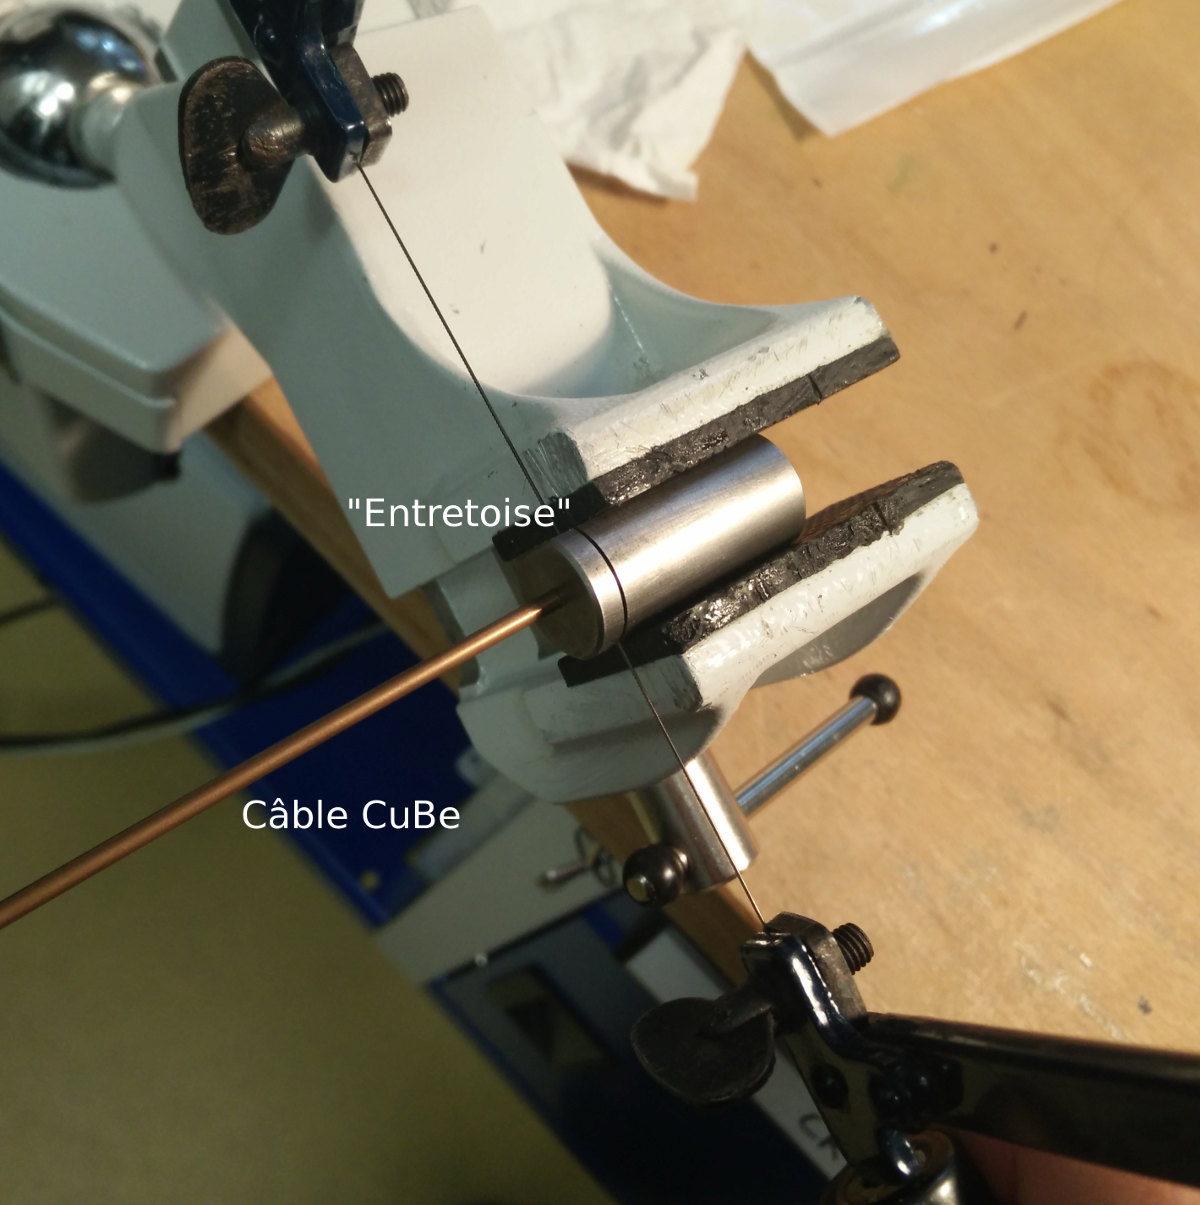
\includegraphics[height=0.48\textwidth]{Images/Coax/1}
        \quad
        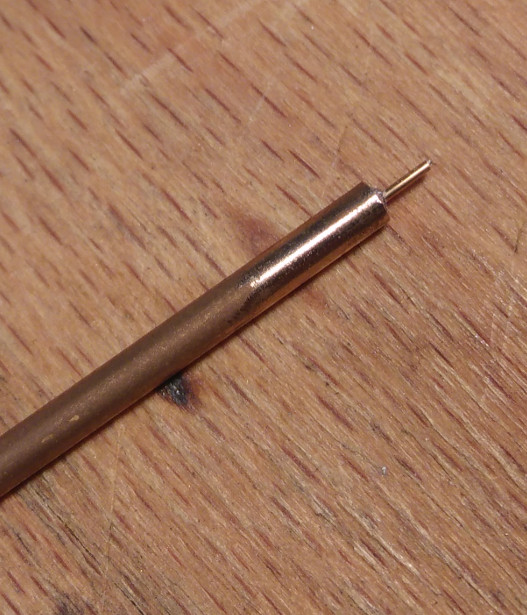
\includegraphics[height=0.48\textwidth]{Images/Coax/2}
        \caption{Dénudage d'un câble coaxial}
        \label{coax_denudage}
    \end{center}
\end{figure}


\paragraph*{Soudure de la pin centrale} 
On fixe la pin sur l'âme du câble, puis on serre le tout en place avec la pièce \textbf{W60}.
     
Pour souder il suffit de chauffer l'extérieur de la pin tout en positionnant le fil d'étain sur le trou sur le bord de la pin.
On fixe une broche sur l’âme du câble, puis on serre le tout en place.

Pour prévoir la dilatation du diélectrique lors de la soudure, on place une petite entretoise \textbf{W56} juste avant la broche.
\begin{figure}[h]
    \begin{center}
        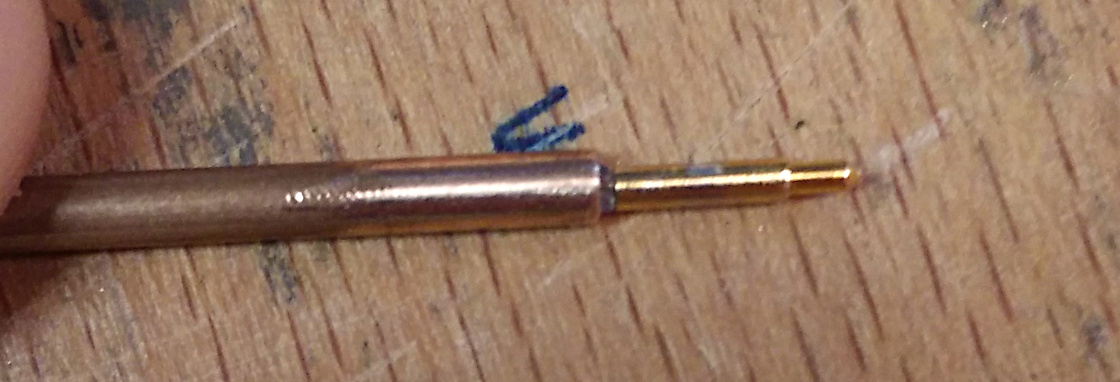
\includegraphics[width=0.60\textwidth]{Images/Coax/3}
        \caption{Pin centrale soudée sur le câble}
        \label{coax_soudure_centre}
    \end{center}
\end{figure}


\paragraph*{Soudure de la prise extérieure} On fixe sur la prise mâle une prise femelle factice \textbf{W14M (81)} qui permet de positionner à la distance correcte la prise mâle. Celle-ci comporte la partie mobile avec le pas de vis.

Le plus efficace est de faire un tortillon d'étain au-dessus de la prise, que l'on chauffe. En étant un peu patient l'étain va fondre et rentrer naturellement dans la prise.

\begin{figure}[ht]
    \begin{center}
        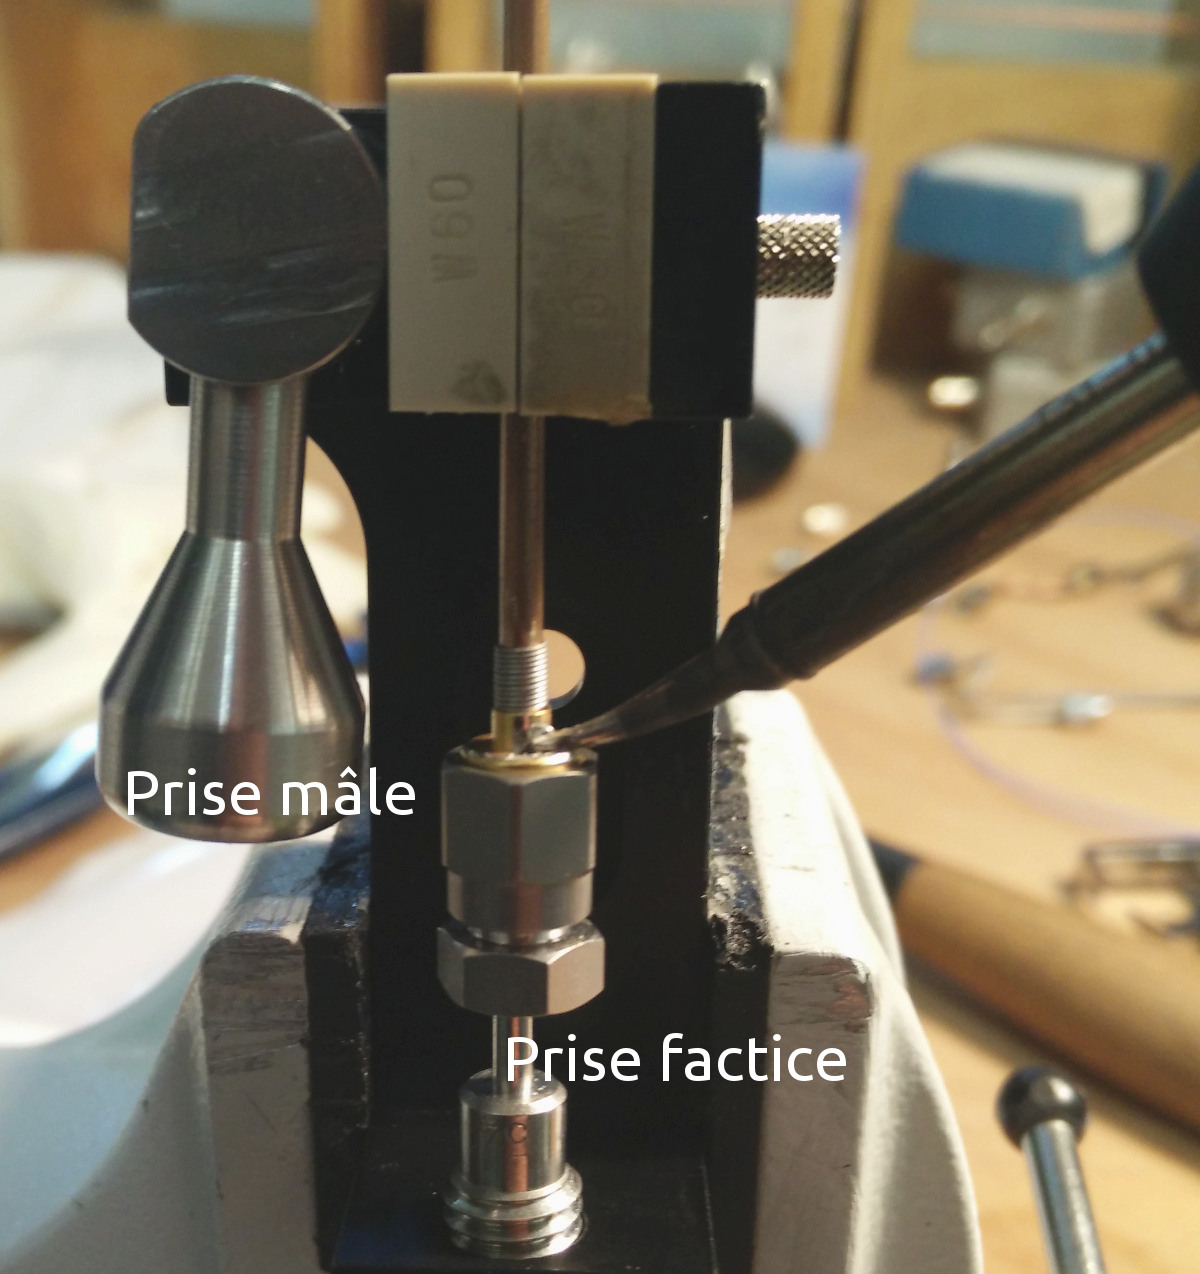
\includegraphics[height=0.48\textwidth]{Images/Coax/4}
        \quad
        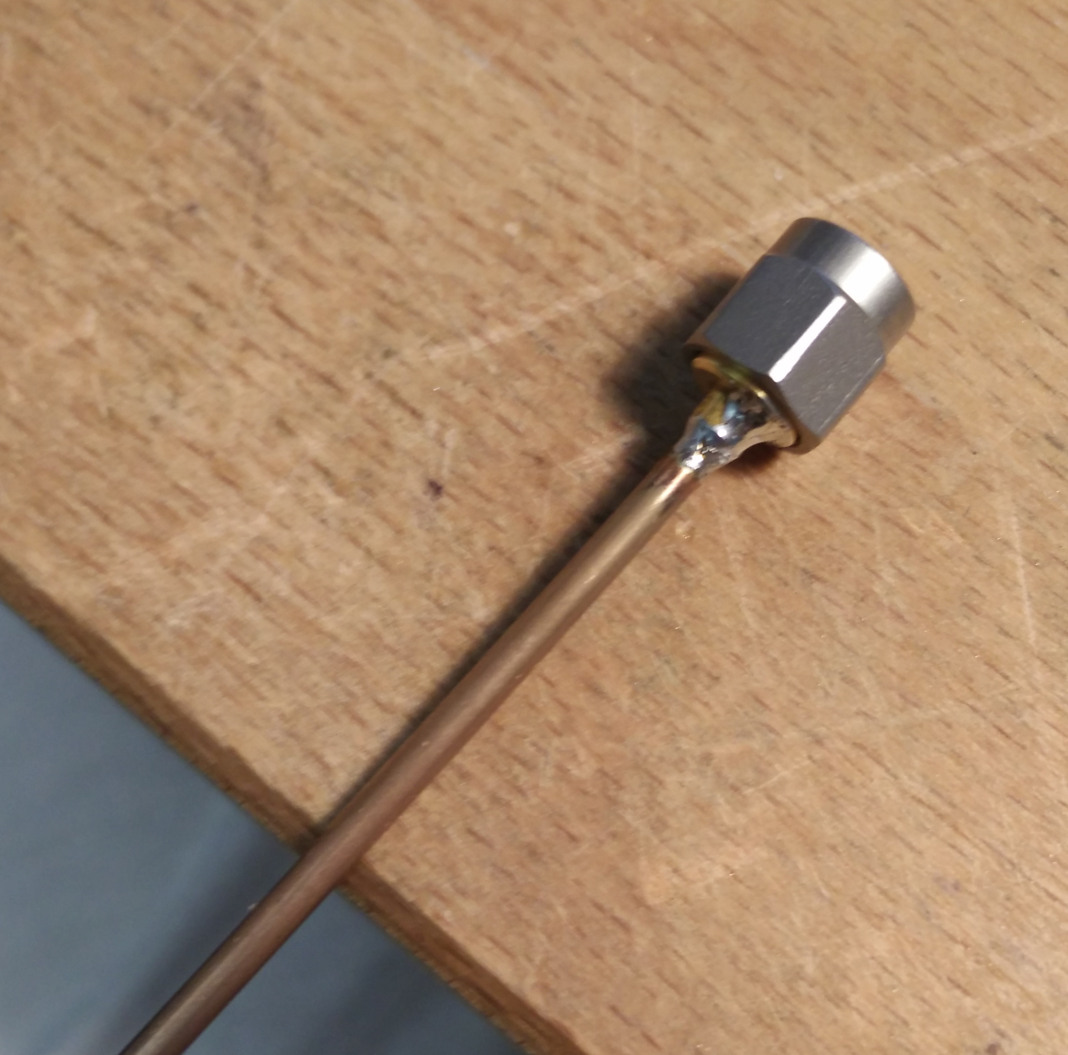
\includegraphics[height=0.48\textwidth]{Images/Coax/5}
        \caption{Soudure de la prise extérieure}
        \label{coax_soudure_exterieur}
    \end{center}
\end{figure}


\newpage
\paragraph*{Fixation de l’isolant}  La dernière étape est de mettre un petit cylindre diélectrique entre la prise et la broche.

On utilise alors la pièce creuse et son "burin" associé \textbf{W52 (W53)} que l'on serre à la clé dynamométrique dans le connecteur pour enfoncer le diélectrique. On place l'isolant à l'intérieur, et on pousse d'un coup avec le "burin".
\begin{figure}[ht]
    \begin{center}
        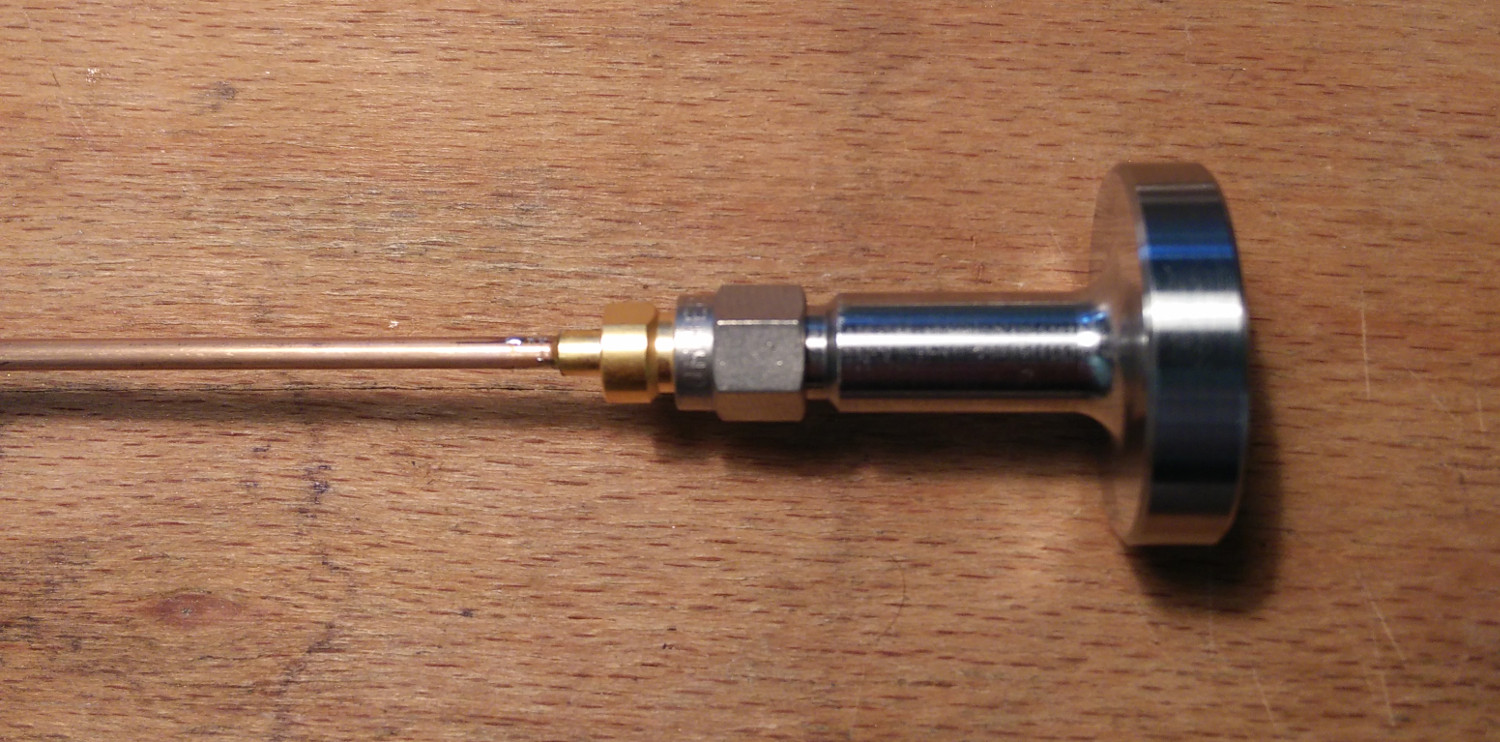
\includegraphics[width=0.60\textwidth]{Images/Coax/6}
        \caption{Fixation de l’isolant}
        \label{coax_fixation_isolant}
    \end{center}
\end{figure}



\paragraph*{Cintrage des câbles coaxiaux} Comme évoqué plus haut, les câbles doivent être cintrés entre chaque étage du cryostat. Néanmoins la fragilité des câbles nous impose de respecter un rayon de courbure minimal de 9mm.

Une cintreuse "sur mesure" permet de cintrer les câble correctement.

On utilise la cintreuse. Pour chaque câble il faut faire un "U" pour éviter les interférences d'un étage à l'autre, et pour avoir une certaine souplesse du câble.

Pour faire : 
\begin{itemize}
    \item $1/4$ tour : il faut 15mm de câble
    \item $1/2$ tour : il faut 29mm
\end{itemize}
Un cintrage en "U" nécessite alors 35mm de câble de plus qu'un câble droit.


\begin{figure}[h]
    \begin{center}
        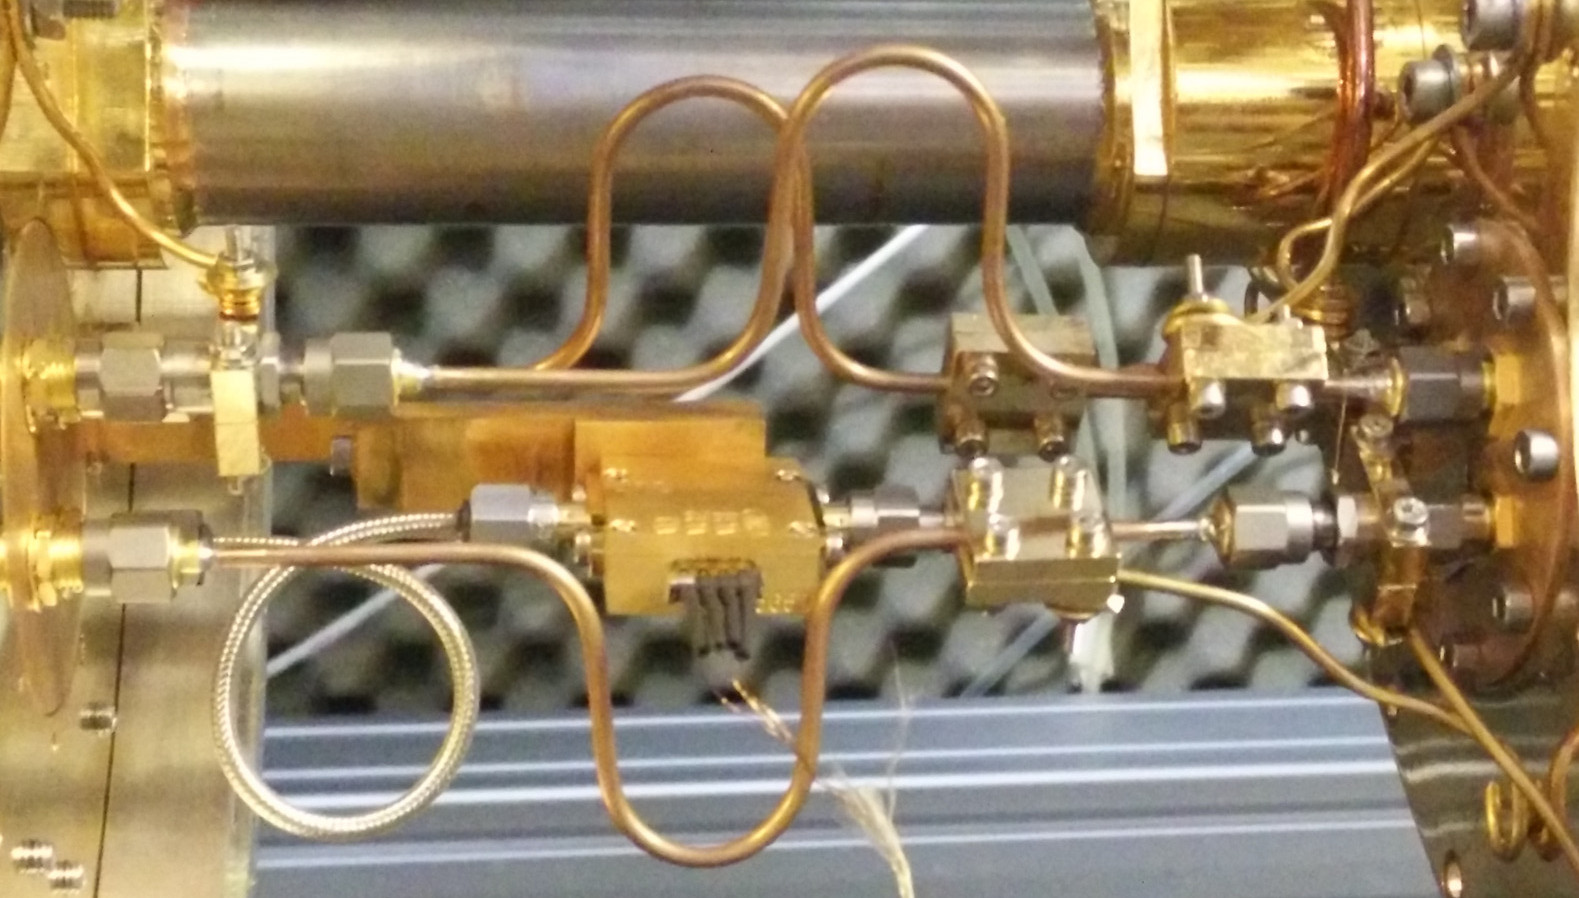
\includegraphics[width=0.65\textwidth]{Images/Coax/cintrage}
        \caption{Câbles coaxiaux cintrés en "U" et connectés}
        \label{coax_cintrage}
    \end{center}
\end{figure}

\newpage
\paragraph*{Mesure du câble nécessaire} Après avoir connectorisé une extrémité du câble, il faut mesurer précisément la longueur de câble nécessaire. Il faut alors prendre en compte la longueur de câble qui se trouve dans le connecteur (sinon, il manquera quelques millimètres).
%TODO Retrouver les mesures exactes

\begin{center}
    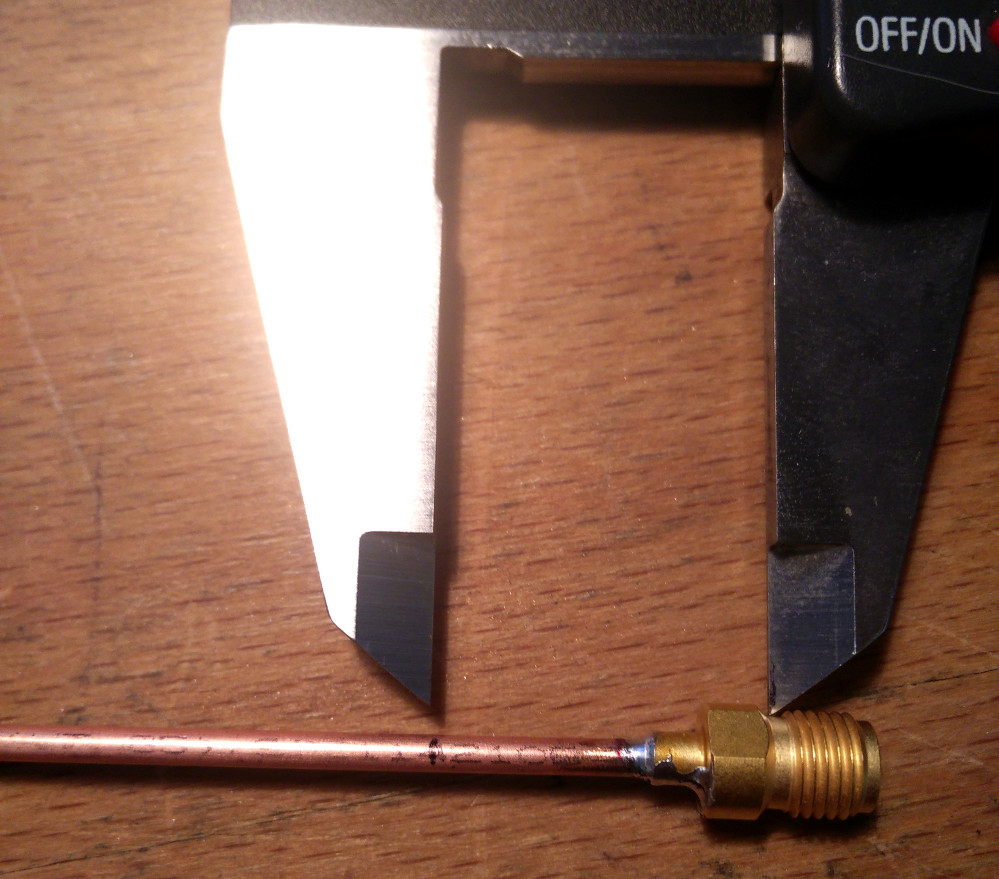
\includegraphics[width=0.40\textwidth]{Images/Coax/mesure}
    \label{coax_mesure}
\end{center}



\subsection{Thermalisation des câbles RF}
Les câbles coaxiaux doivent être thermalisés à chaque étage du cryostat par les pinces dorées (sur les câbles \textit{et} sur les atténuateurs), reliées par des câbles de cuivre jusqu’aux platines du cryostat.

Les câbles RF se thermalisent grâce aux pinces dorées . On utilise l'Apiezon N pour avoir un bon contact thermique avec la pince, en comblant les pores des parois en contact.

Une des vis de chaque pince permet de fixer un fil de cuivre doré (elle est donc plus longue que les autres).

\begin{description}
    \item[Sur câble RG405 :] 3 vis 10mm + 1 vis 16mm
    \item[Sur atténuateur :] 1 vis 16mm + 1 vis 2mm
\end{description}
